% \documentclass[a4paper,landscape]{article}

\documentclass{standalone}

\usepackage[svgnames]{xcolor}
\usepackage{tikz}
\usetikzlibrary{calc}
\usetikzlibrary{decorations.markings}
\usetikzlibrary{shapes.geometric}
\usetikzlibrary{patterns}

\pgfdeclarelayer{edgelayer}
\pgfdeclarelayer{nodelayer}
\pgfsetlayers{edgelayer,nodelayer,main}

\tikzstyle{none}=[inner sep=0pt]


%---------------------------------------------------
% Node styles
%---------------------------------------------------
\tikzstyle{ouput_layer_unit}=[fill={rgb,255: red,70; green,129; blue,255}, draw={rgb,255: red,8; green,0; blue,249}, shape=circle]

\tikzstyle{hidden_layer_unit}=[fill={rgb,255: red,147; green,255; blue,255}, draw={rgb,255: red,58; green,123; blue,180}, shape=circle]

\tikzstyle{empty_slot}=[fill=white, draw=black, shape=circle]

\tikzstyle{output_1} = [preaction={fill={rgb,255: red,70 ; green,129; blue,255}}, pattern color=black, pattern=north west lines, draw={rgb,255: red,8; green,0; blue,249}, shape=circle]
\tikzstyle{output_2} = [preaction={fill={rgb,255: red,70 ; green,129; blue,255}}, pattern color=black, pattern=dots, draw={rgb,255: red,8; green,0; blue,249}, shape=circle]
\tikzstyle{output_3} = [preaction={fill={rgb,255: red,70 ; green,129; blue,255}}, pattern color=black, pattern=north east lines, draw={rgb,255: red,8; green,0; blue,249}, shape=circle]
\tikzstyle{output_4} = [preaction={fill={rgb,255: red,70 ; green,129; blue,255}}, pattern color=black, pattern=grid, draw={rgb,255: red,8; green,0; blue,249}, shape=circle]

\tikzstyle{parameter_vector_unit}=[fill={rgb,255: red,255; green,0; blue,4}, draw={rgb,255: red,107; green,0; blue,1}, shape=circle]

\tikzstyle{myText}=[fill=white, draw=white, shape=rectangle]

\tikzstyle{ellipsis}=[fill=black, draw=black, shape=circle]

\tikzstyle{rectangle}=[fill={rgb,255: red,98; green,255; blue,161}, draw=black, shape=rectangle]

%---------------------------------------------------
% Edge styles
%---------------------------------------------------
\tikzstyle{section_marker}=[{|-|}]
\tikzstyle{main_connector}=[-, draw={rgb,255: red,184; green,184; blue,184}]
\tikzstyle{secondary_concetor}=[-, draw={rgb,255: red,176; green,204; blue,229}, dashed]

\definecolor{my_pink}{HTML}{f2e6ff}
\definecolor{my_purple}{HTML}{6600CC}
\definecolor{dark_green}{HTML}{0C5600}

\begin{document}

\pagestyle{empty}

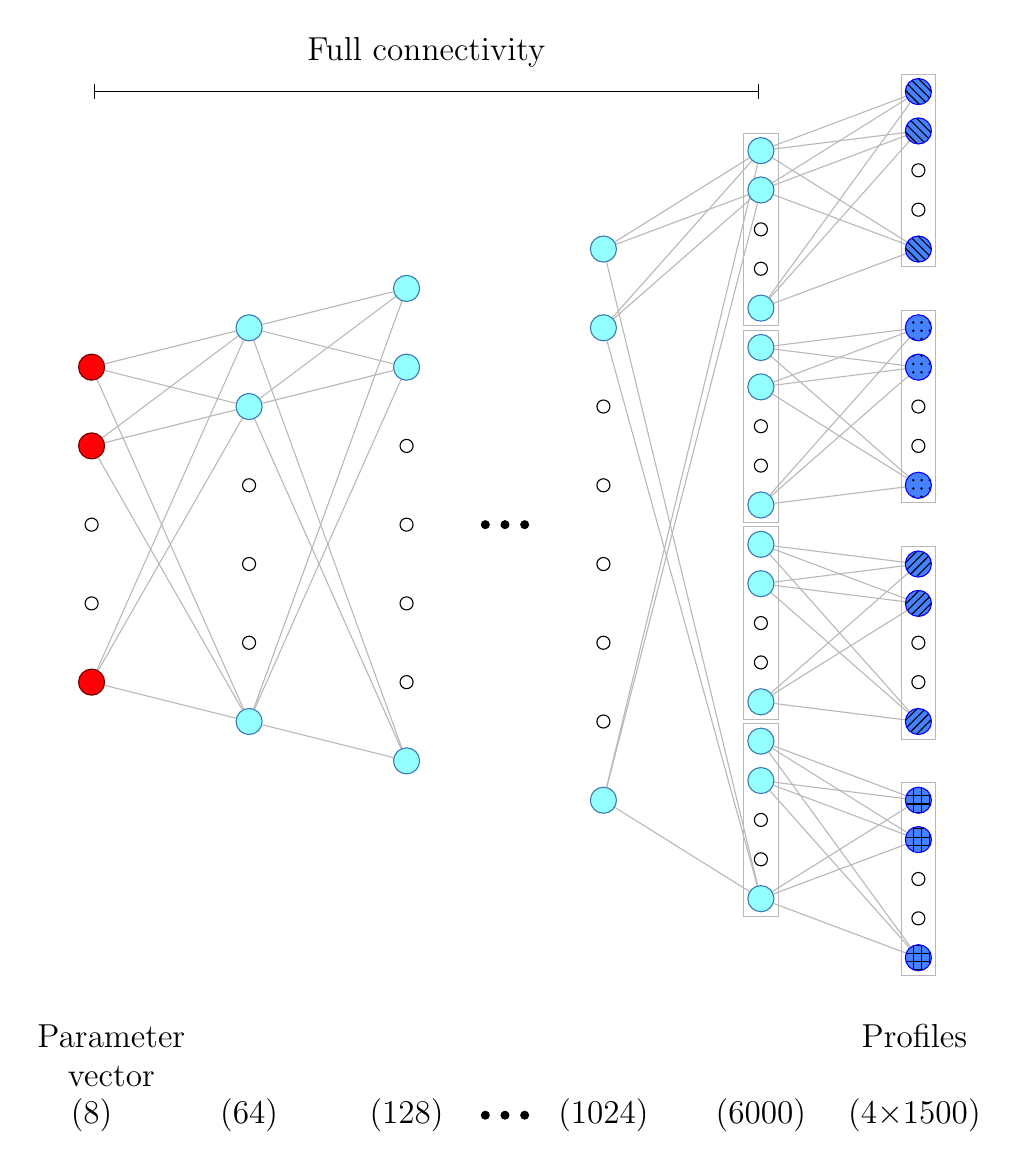
\begin{tikzpicture}
    \begin{pgfonlayer}{nodelayer}
        % input layer
        \node [style={parameter_vector_unit}] (0) at (0, 0) {};
        \node [style={parameter_vector_unit}] (3) at (0, 3) {};
        \node [style={parameter_vector_unit}] (4) at (0, 4) {};
        \node [style={empty_slot}, scale=0.5] (5) at (0, 2) {};
        \node [style={empty_slot}, scale=0.5] (6) at (0, 1) {};

        % first hidden layer
        \node [style={hidden_layer_unit}] (7) at (2, 4.5) {};
        \node [style={hidden_layer_unit}] (8) at (2, 3.5) {};
        \node [style={hidden_layer_unit}] (9) at (2, -0.5) {};
        \node [style={empty_slot}, scale=0.5] (11) at (2, 2.5) {};
        \node [style={empty_slot}, scale=0.5] (12) at (2, 1.5) {};
        \node [style={empty_slot}, scale=0.5] (13) at (2, 0.5) {};
        
        % second hidden layer
        \node [style={hidden_layer_unit}] (17) at (4, 5) {};
        \node [style={hidden_layer_unit}] (18) at (4, 4) {};
        \node [style={hidden_layer_unit}] (19) at (4, -1) {};
        \node [style={empty_slot}, scale=0.5] (21) at (4, 3) {};
        \node [style={empty_slot}, scale=0.5] (22) at (4, 2) {};
        \node [style={empty_slot}, scale=0.5] (23) at (4, 1) {};
        \node [style={empty_slot}, scale=0.5] (24) at (4, 0) {};

        % ellipsis    
        \node [style=ellipsis, scale=0.3] (34) at (5.0, 2) {};
        \node [style=ellipsis, scale=0.3] (35) at (5.25, 2) {};
        \node [style=ellipsis, scale=0.3] (36) at (5.5, 2) {};
        
        % hidden layer
        \node [style={hidden_layer_unit}] (37) at (6.5, 4.5) {};
        \node [style={hidden_layer_unit}] (38) at (6.5, 5.5) {};
        \node [style={hidden_layer_unit}] (39) at (6.5, -1.5) {};
        \node [style={empty_slot}, scale=0.5] (29) at (6.5, 3.5) {};
        \node [style={empty_slot}, scale=0.5] (30) at (6.5, 2.5) {};
        \node [style={empty_slot}, scale=0.5] (31) at (6.5, 1.5) {};
        \node [style={empty_slot}, scale=0.5] (32) at (6.5, 0.5) {};
        \node [style={empty_slot}, scale=0.5] (33) at (6.5, -0.5) {};

        % final hidden layer
%         \node [style=hidden_layer_unit] (40) at (8.5, 6) {};
%         \node [style=hidden_layer_unit] (41) at (8.5, 5) {};
%         \node [style=hidden_layer_unit] (42) at (8.5, -2) {};
%         \node [style={empty_slot}, scale=0.5] (43) at (8.5, 4) {};
%         \node [style={empty_slot}, scale=0.5] (44) at (8.5, 3) {};
%         \node [style={empty_slot}, scale=0.5] (45) at (8.5, 2) {};
%         \node [style={empty_slot}, scale=0.5] (46) at (8.5, 1) {};
%         \node [style={empty_slot}, scale=0.5] (47) at (8.5, 0) {};
%         \node [style={empty_slot}, scale=0.5] (48) at (8.5, -1) {};
        

        % output layer (4x1500 units)
        %1
        \node [style={hidden_layer_unit}]       (h11)   at (8.5, 6.75) {};
        \node [style={hidden_layer_unit}]       (h12)   at (8.5, 6.25) {};
        \node [style={empty_slot}, scale=0.5]   (h13)   at (8.5, 5.75) {};
        \node [style={empty_slot}, scale=0.5]   (h14)   at (8.5, 5.25) {};  
        \node [style={hidden_layer_unit}]       (h15)   at (8.5, 4.75) {};
        %2                                                  
        \node [style={hidden_layer_unit}]       (h21)   at (8.5, 4.25) {};
        \node [style={hidden_layer_unit}]       (h22)   at (8.5, 3.75) {};
        \node [style={empty_slot}, scale=0.5]   (h23)   at (8.5, 3.25) {};
        \node [style={empty_slot}, scale=0.5]   (h24)   at (8.5, 2.75) {};  
        \node [style={hidden_layer_unit}]       (h25)   at (8.5, 2.25) {};        
        %3                                                  
        \node [style={hidden_layer_unit}]       (h31)   at (8.5, 1.75) {};
        \node [style={hidden_layer_unit}]       (h32)   at (8.5, 1.25) {};
        \node [style={empty_slot}, scale=0.5]   (h33)   at (8.5, 0.75) {};
        \node [style={empty_slot}, scale=0.5]   (h34)   at (8.5, 0.25) {};  
        \node [style={hidden_layer_unit}]       (h35)   at (8.5, -0.25) {};        
        %4                                                  
        \node [style={hidden_layer_unit}]       (h41)   at (8.5, -0.75) {};
        \node [style={hidden_layer_unit}]       (h42)   at (8.5, -1.25) {};
        \node [style={empty_slot}, scale=0.5]   (h43)   at (8.5, -1.75) {};
        \node [style={empty_slot}, scale=0.5]   (h44)   at (8.5, -2.25) {};  
        \node [style={hidden_layer_unit}]       (h45)   at (8.5, -2.75) {};         
        
        % output layer (4x1500 units)
        %1
        \node [style={output_1}]                (o11)   at (10.5, 7.5) {};
        \node [style={output_1}]                (o12)   at (10.5, 7.0) {};
        \node [style={empty_slot}, scale=0.5]   (o13)   at (10.5, 6.5) {};
        \node [style={empty_slot}, scale=0.5]   (o14)   at (10.5, 6.0) {};  
        \node [style={output_1}]                (o15)   at (10.5, 5.5) {};
        %2                                                   
        \node [style={output_2}]                (o21)   at (10.5, 4.5) {};
        \node [style={output_2}]                (o22)   at (10.5, 4.0) {};
        \node [style={empty_slot}, scale=0.5]   (o23)   at (10.5, 3.5) {};
        \node [style={empty_slot}, scale=0.5]   (o24)   at (10.5, 3.0) {};  
        \node [style={output_2}]                (o25)   at (10.5, 2.5) {};        
        %3                                                   
        \node [style={output_3}]                (o31)   at (10.5, 1.5) {};
        \node [style={output_3}]                (o32)   at (10.5, 1.0) {};
        \node [style={empty_slot}, scale=0.5]   (o33)   at (10.5, 0.5) {};
        \node [style={empty_slot}, scale=0.5]   (o34)   at (10.5, 0.0) {};  
        \node [style={output_3}]                (o35)   at (10.5, -0.5) {};        
        %4                                                   
        \node [style={output_4}]                (o41)   at (10.5, -1.5) {};
        \node [style={output_4}]                (o42)   at (10.5, -2.0) {};
        \node [style={empty_slot}, scale=0.5]   (o43)   at (10.5, -2.5) {};
        \node [style={empty_slot}, scale=0.5]   (o44)   at (10.5, -3.0) {};  
        \node [style={output_4}]                (o45)   at (10.5, -3.5) {};                    
        
        
        % description at the bottom 
        \node [style=myText] (50) at (0, -5.5) {\large (8)};
        \node [style=myText] (51) at (0.25, -4.5) {\large Parameter};
        \node [style=myText] (52) at (0.25, -5.0) {\large vector};
        
        
        \node [style=myText] (58) at (2, -5.5) {\large (64)};
        \node [style=myText] (59) at (4, -5.5) {\large (128)};
        
        % ellipsis    
        \node [style=ellipsis, scale=0.3] (59a) at (5.0, -5.5) {};
        \node [style=ellipsis, scale=0.3] (59b) at (5.25, -5.5) {};
        \node [style=ellipsis, scale=0.3] (59c) at (5.5, -5.5) {};
        
        \node [style=myText] (60) at (6.5, -5.5) {\large (1024)};
        \node [style=myText] (61) at (8.5, -5.5) {\large (6000)};
        \node [style=myText] (62) at (10.45, -5.5) {\large (4$\times$1500)};
        \node [style=myText] (63) at (10.45, -4.5) {\large Profiles};
        
        
        % text at the top
        \node [style=myText] (55) at (4.25, 8.0) {\large Full connectivity};
        % epmty nodes for docking line at the top 
        \node [style=none] (100) at (0.0,  7.5) {};
        \node [style=none] (101) at (8.5,  7.5) {};
        
    \end{pgfonlayer}
    \begin{pgfonlayer}{edgelayer}
        \draw [style={main_connector}] (4) to (7);
        \draw [style={main_connector}] (4) to (8);
        \draw [style={main_connector}] (4) to (9);
        \draw [style={main_connector}] (3) to (7);
        \draw [style={main_connector}] (3) to (8);
        \draw [style={main_connector}] (3) to (9);
        \draw [style={main_connector}] (0) to (9);
        \draw [style={main_connector}] (0) to (8);
        \draw [style={main_connector}] (0) to (7);
        \draw [style={main_connector}] (7) to (17);
        \draw [style={main_connector}] (7) to (18);
        \draw [style={main_connector}] (8) to (18);
        \draw [style={main_connector}] (8) to (17);
        \draw [style={main_connector}] (7) to (19);
        \draw [style={main_connector}] (8) to (19);
        \draw [style={main_connector}] (19) to (9);
        \draw [style={main_connector}] (9) to (18);
        \draw [style={main_connector}] (9) to (17);
%         \draw [style={main_connector}] (38) to (40);
%         \draw [style={main_connector}] (38) to (41);
%         \draw [style={main_connector}] (37) to (40);
%         \draw [style={main_connector}] (38) to (42);
%         \draw [style={main_connector}] (42) to (39);
%         \draw [style={main_connector}] (39) to (41);
%         \draw [style={main_connector}] (40) to (39);
%         \draw [style={main_connector}] (37) to (41);
%         \draw [style={main_connector}] (37) to (42);



        \draw [style={main_connector}] (38) to (h11);
        \draw [style={main_connector}] (38) to (h12);
        \draw [style={main_connector}] (38) to (h45);

               
        \draw [style={main_connector}] (37) to (h11);
        \draw [style={main_connector}] (37) to (h12);
        \draw [style={main_connector}] (37) to (h45);
        
        \draw [style={main_connector}] (39) to (h11);
        \draw [style={main_connector}] (39) to (h12);
        \draw [style={main_connector}] (39) to (h45);
        
        
        \draw [style={section_marker}] (100) to (101);
        
        % 1: connections between final hidden and output layer
        \draw [style={main_connector}] (h11) to (o11);
        \draw [style={main_connector}] (h12) to (o11);
        \draw [style={main_connector}] (h15) to (o11);        
        \draw [style={main_connector}] (h11) to (o12);
        \draw [style={main_connector}] (h12) to (o12);
        \draw [style={main_connector}] (h15) to (o12);
        \draw [style={main_connector}] (h11) to (o15);
        \draw [style={main_connector}] (h12) to (o15);
        \draw [style={main_connector}] (h15) to (o15);
        
        % 2: connections between final hidden and output layer
        \draw [style={main_connector}] (h21) to (o21);
        \draw [style={main_connector}] (h22) to (o21);
        \draw [style={main_connector}] (h25) to (o21);        
        \draw [style={main_connector}] (h21) to (o22);
        \draw [style={main_connector}] (h22) to (o22);
        \draw [style={main_connector}] (h25) to (o22);
        \draw [style={main_connector}] (h21) to (o25);
        \draw [style={main_connector}] (h22) to (o25);
        \draw [style={main_connector}] (h25) to (o25);
       
        % 3: connections between final hidden and output layer
        \draw [style={main_connector}] (h31) to (o31);
        \draw [style={main_connector}] (h32) to (o31);
        \draw [style={main_connector}] (h35) to (o31);        
        \draw [style={main_connector}] (h31) to (o32);
        \draw [style={main_connector}] (h32) to (o32);
        \draw [style={main_connector}] (h35) to (o32);
        \draw [style={main_connector}] (h31) to (o35);
        \draw [style={main_connector}] (h32) to (o35);
        \draw [style={main_connector}] (h35) to (o35);
        
        % 4: connections between final hidden and output layer
        \draw [style={main_connector}] (h41) to (o41);
        \draw [style={main_connector}] (h42) to (o41);
        \draw [style={main_connector}] (h45) to (o41);        
        \draw [style={main_connector}] (h41) to (o42);
        \draw [style={main_connector}] (h42) to (o42);
        \draw [style={main_connector}] (h45) to (o42);
        \draw [style={main_connector}] (h41) to (o45);
        \draw [style={main_connector}] (h42) to (o45);
        \draw [style={main_connector}] (h45) to (o45);            
        
        
        % draw 4 boxes around the final hidden layers
        \draw[draw={rgb,255: red,184; green,184; blue,184}, line width=0.1mm] ($(h11.north west)+(-0.1,0.1)$) rectangle ($(h15.south east)+(0.1,-0.1)$);
        \draw[draw={rgb,255: red,184; green,184; blue,184}, line width=0.1mm] ($(h21.north west)+(-0.1,0.1)$) rectangle ($(h25.south east)+(0.1,-0.1)$);
        \draw[draw={rgb,255: red,184; green,184; blue,184}, line width=0.1mm] ($(h31.north west)+(-0.1,0.1)$) rectangle ($(h35.south east)+(0.1,-0.1)$);
        \draw[draw={rgb,255: red,184; green,184; blue,184}, line width=0.1mm] ($(h41.north west)+(-0.1,0.1)$) rectangle ($(h45.south east)+(0.1,-0.1)$);
        
        % draw 4 boxes around the final hidden layers
        \draw[draw={rgb,255: red,184; green,184; blue,184}, line width=0.1mm] ($(o11.north west)+(-0.1,0.1)$) rectangle ($(o15.south east)+(0.1,-0.1)$);
        \draw[draw={rgb,255: red,184; green,184; blue,184}, line width=0.1mm] ($(o21.north west)+(-0.1,0.1)$) rectangle ($(o25.south east)+(0.1,-0.1)$);
        \draw[draw={rgb,255: red,184; green,184; blue,184}, line width=0.1mm] ($(o31.north west)+(-0.1,0.1)$) rectangle ($(o35.south east)+(0.1,-0.1)$);
        \draw[draw={rgb,255: red,184; green,184; blue,184}, line width=0.1mm] ($(o41.north west)+(-0.1,0.1)$) rectangle ($(o45.south east)+(0.1,-0.1)$);
        
    \end{pgfonlayer}
\end{tikzpicture}

\end{document}
